\chapter{Introduction}

\begin{quote}
``There are infinite worlds both like and unlike this world of
ours. For the atoms being infinite in number, as was already proven,
...there nowhere exists an obstacle to the infinite number of worlds.''
\end{quote}
\hfill Epicurus ($\sim$341-270 B.C.)

\begin{comment}
\begin{quote}
``This space we declare to be infinite... In it are an infinity of
worlds of the same kind as our own.''
\end{quote}
\hfill Giordano Bruno, {\it On the Inifinite Universe and Worlds} (1584)
\end{comment}

\begin{quote}
``How vast those Orbs must be, and how inconsiderable this Earth, the
Theatre upon which all our mighty Designs, all our Navigations, and
all our Wars are transacted, is when compared to them.''
\end{quote}
\hfill Christiaan Huygens, {\it Cosmotheoros} (1698)

\begin{quote}
``Of all of the topics of study in astronomy, exoplanets hold a
special place in the imagination. More than stars, nebulae, or
galaxies, they are {\it places}, ...''
\end{quote}
\hfill \cite{2006PhDT.........8W}

%%%%%%%%%%%%%%%%%%%%%%%%%%%%%%%%%%%%%%%%%%%%%%%%%%%%%%%%%%%%%%%%%%%%%%%%%%%%%%
\section{On Detecting New Worlds}

Even before human beings realized that other stars are like our Sun,
the existence of other worlds have been speculated by ancient greek
philosophers such as Epicurus and Democritus. In the blooming age of
astronomy in the 1400s and 1600s, early pioneers such as Giordano
Bruno and Christiaan Huygens have also pondered upon the existence of
planets around other stars (extra-solar planets, or
exoplanets).\footnote{In fact, Huygens conducted the first documented
search on exoplanets. For more on the history of exoplanet searches,
see these three websites:\\ The NASA PlanetQuest,
http://www.nasa.gov/externalflash/PQTimeline/; \\ Search for
Exoplanets, http://www.hao.ucar.edu/research/stare/search.html; \\
ESO,
https://www.eso.org/public/outreach/eduoff/cas/cas2004/casreports-2004/rep-228/. }
In modern times, 40 years before the discovery of the first exoplanet,
Otto Struve stated that exoplanets, especially ``super-Jupiters'' on
short orbits, should be detectable via spectroscopy and photometry
\citep{1952Obs....72..199S}.

Unfortunately, the earliest claims of exoplanet detections before
1980s all turned out to be erroneous \citep{1855MNRAS..15..228J,
1969AJ.....74..757V}. These and a later retracted claim of a planet
around a pulsar by \cite{1991Natur.352..311B} made all astronomers
extremely cautious about exoplanet detection claims. In 1988,
Campbell, Walker and Yang announced potential planetary signal from
the star Gamma Cephei, but they were hesitant in calling it a
detection due to limitations of early instruments. Their detection
method was to measure the radial velocity (RV) variation of the star
using precise Doppler spectroscopy, which is described in the next
section and is also the theme of this thesis.  It was not until 2003
that the planet around $\gamma$ Cephei A was confirmed
\citep{2003ApJ...599.1383H}, which made the work of
\cite{1988ApJ...331..902C} the first exoplanet detection. The
detection of HD 114762b (``Latham Planet'';
\citealt{1989Natur.339...38L}) also belongs to the family of first
exoplanet detections, though the planet was thought to be a brown
dwarf at the time due to its large mass. A similar story to $\gamma$
Cephei Ab is the discovery of $\beta$ Gemini b
\citep{1993ApJ...413..339H}, where the existence of the planet was not
confirmed until 2006 \citep{2006A&A...457..335H} because of the strong
activity-induced RV signals of the giant host star.\footnote{See
  Chapter 4 of \cite{2013pss3.book..489W} for a more detailed history
  on these early detections.} 

The more commonly recognized first detection of exoplanets belongs to
\cite{1993ApJ...413..339H}, who reported two planets around the pulsar
PSR B1257$+$12, detected via the pulsar timing method using radio data
(later on it turned out this system hosts one more planet). It was a
surprising detection in many aspects, and these planets remains the
only known planetary system around a pulsar to date (as of May
2016). If exoplanets could exist around exotic stars like pulsars,
then it is only natural to expect them to exist around more
``regular'' main-sequence stars like our Sun.

Finally, in 1995, a team in Geneva announced the first definitive
detection of a planet around a main-sequence star, 51 Peg b
\citep{1995Natur.378..355M}. Their results were quickly confirmed by
other planet hunters such as Geoffrey W.\ Marcy and R.\ Paul Butler,
who quickly caught up with the game \citep{1996ApJ...464L.153B} and
went on to detect more than half of the hundreds of known exoplanets
up until the launch of NASA's \kepler\ mission
\cite{2010Sci...327..977B}. The method adopted by
\cite{1995Natur.378..355M} and \cite{1996ApJ...464L.153B} was again
precise Doppler spectroscopy. Today, there are over 585 exoplanets
discovered by precise Doppler spectroscopy. The discoveries by precise
Doppler spectroscopy that happened beyond this point is briefly
accounted for in the next section. 

Several years later, \cite{2000ApJ...529L..41H} and
\cite{2000ApJ...529L..45C} detected the first exoplanet transiting
event, where the planet moves in between the disk of the star and our
line of sight periodically, leaving signals in the stellar light
curves. This transiting planet, HD 209458b, which was discovered via
precise Doppler spectroscopy first. Nonetheless, this discovery opened
up the age of transit detections, where projects such as OGLE, TrES,
WASP, XO, HAT, and CoRoT etc.\ added more than 200 new exoplanet
discoveries to date \citep{2003Natur.421..507K, 2004ApJ...613L.153A,
2006MNRAS.372.1117C, 2006ApJ...648.1228M, 2007ApJ...656..552B}.

In 2009, the discovery of exoplanets entered a new era with the launch
of NASA's \kepler\ satellite, which is a dedicated space mission to
detect transiting exoplanets. This extremely fruitful mission has made
new exoplanet discoveries in the counts of thousands
\citep{2014ApJ...784...45R, 2016ApJ...822...86M}, with over 2000 more
planet candidates (see, e.g., NASA Exoplanet Archive for statistics on
exoplanet discoveries). The science of exoplanets expanded from the
philatelic style to including population and statistical studies which
inform planet formation and evolution in powerful ways more than ever
(e.g., \citealt{2013ApJ...766...81F} on occurrence rate and
\citealt{2015arXiv150407557W} on composition distribution). As of May
23 2016, there are 3268 confirmed exoplanets, to which the transit
method contributed 2569 (585 discovered by Doppler spectroscopy).

Besides using precise Doppler spectroscopy and transits, other methods
have also made unique and important discoveries of exoplanets, as they
probe different stellar population and are subject to different
observational biases. \cite{2004ApJ...606L.155B} made the first
micro-lensing detection of exoplanet, where planets acts as additional
gravitational lenses beside their host star and leave characteristic
signatures onto the light curves of the background star. There are 37
exoplanets discovered via micro-lensing so far. Astronomers also
directly detected light from young exoplanets around young stars via
direct imaging, the first of which are Fomalhaut b
\citep{2008Sci...322.1345K} and the four planets around HR 8799
\citep{2008Sci...322.1348M}. Today, there are 41 directly imaged
planets.

More exoplanets around more diverse host stars are expected to be
discovered in the near future, with many new missions and surveys
being carried out, built, or planned. Post-2013, \kepler\ continued as
the K2 mission (\kepler\ on two reaction wheels) and kept churning out
planets (e.g., \citealt{2016ApJS..222...14V}). The Transiting
Exoplanet Survey Satellite (TESS; \citealt{2014SPIE.9143E..20R};
expected to launch in Summer 2017) will survey the whole sky,
targeting nearby and bright stars, including the previously relatively
unexplored population of M dwarf stars. There is no doubt that, once
again, exoplanet discoveries will be made in counts of
thousands. Ongoing surveys with the Gemini Planet Imager on Gemini
South \citep{2014PNAS..11112661M} and the SPHERE instrument on the
Very Large Telescope \citep{2008SPIE.7014E..18B} are populating
exoplanets in a new parameter space (young stellar/planetary age and
moderate to long orbital distances). The future for micro-lensing
discoveries also remains bright as thousands of exoplanets are
expected to be found by NASA's WFIRST-AFTA mission
\citep{2014arXiv1409.2759Y}.

Among all these exciting discoveries happening or on the horizon,
precise Doppler spectroscopy continues to play an important role. It
is the most important method for measuring planetary
masses,\footnote{Planetary masses can also be measured via studies on
the transit timing variations (TTVs) due to the dynamic interactions
of multiple planets (e.g., \citealt{2016ApJ...820...39J}), but TTVs
are only measurable for a small fraction of all transiting planets
\citep{mazeh2013}. \cite{2013Sci...342.1473D} have also developed an
innovative method to estimate planetary mass via transmission
spectroscopy of the planetary atmosphere, but the method is
model-dependent and requires a large amount of large-aperture space
telescope time (e.g., hundreds of orbits of JWST).} and it will remain
a crucial independent method for discovering new exoplanets (after
all, only a small fraction of exoplanets happen to pass in between
their host star and the Earth). The synergy between the \kepler\
mission and the ground-based Doppler spectroscopy follow-ups has
demonstrated the power of this new exoplanet discovery and
characterization ``routine'', where RVs are presented as the
convincing evidence for the planetary nature of the transit signal,
and they also provide valuable information on the planetary masses and
thus their bulk densities (e.g., \citealt{marcy2014}). Such
measurements are crucial for mapping out the demographics of
exoplanets. However, only a small fraction of \kepler\ targets have
been followed up by Doppler spectroscopy, and the future discoveries
of TESS will put an even higher demand on RV follow up (see, e.g.,
a summary in \citealt{exopag2015}).

Doppler spectroscopy also remains the most promising avenue for
detecting Earth-like planet in the Habitable Zone
\citep{1993Icar..101..108K, 2013ApJ...765..131K} in the near
future. Figure~\ref{intro:fig:hz} illustrates the Habitable Zones for
different types of stars and the discovery space that TESS will
access, which does not include the Habitable Zone around Sun-like to
early-M stars due to TESS's short lifespan. The next generation
Doppler spectroscopy, with a RV precision of $<$0.5~m/s, bears great
hope for detecting rocky or even Earth-like planets in the Habitable
Zone. Can we fulfill such a great expectation? The next section
focuses on the art of precise Doppler spectroscopy, on how we achieved
the current precision of 1~m/s today, and on how the field will carry
on and aim for a RV precision of $\sim 10$~cm/s in the coming decade.


%----------------------------------------------------------------
% stellar T vs. planet period, showing RV amplitude curves
% plot provided by Paul Robertson, converted online to eps
\begin{figure}
\centering
\includegraphics[scale=0.55]{introduction/habitable_zone.eps}
\caption{Habitable Zone for stars with various effective temperature,
  highlighted in blue (and red for the extended zone). Some known
  planets in the Habitable Zone of their host stars are plotted, scaled
  by their sizes. Solar system planets are also plotted and scaled by
  size. The yellow and orange dashed vertical lines mark the discovery
  space in terms of planetary periods that TESS is most sensitive
  to. The white curves are equal-RV-amplitude lines, showing the
  semi-amplitude of the RV signals induced by any hypothetical
  Earth-mass planets on each curve. This plot is made by Chester Harman
  and Ravi Kopparapu and kindly provided by Paul Robertson.
\label{intro:fig:hz}}
\end{figure}
%----------------------------------------------------------------



%%%%%%%%%%%%%%%%%%%%%%%%%%%%%%%%%%%%%%%%%%%%%%%%%%%%%%%%%%%%%%%%%%%%%%%%%%%%%%
\section{The Art of Precise Doppler Spectroscopy}

Although it has been common practice to measure the radial velocities
(RVs) of stars for over a century, the idea of measuring them {\it
precisely}, to the order of 10s m/s and below, was first proposed in
1973 by zzz Griffin \& Griffin, where they proposed to use atmospheric
oxygen lines as wavelength calibration and estimated that a precision
of 10~m/s should be attainable. The source of wavelength calibration
and how the calibration is done are two of the key aspects in
measuring precise RVs. From very early on,\footnote{A more detailed
recount on the early history of precise Doppler spectroscopy can be
found in Section 4.3 in \cite{2013pss3.book..489W}.} there have been
two types of ideas, which also heavily shaped the landscapes of
today's precise Doppler spectrometers. One idea uses simultaneous
wavelength calibration, where the spectral lines of the calibrator are
blended with the stellar lines, such as the oxygen lines in the
atmosphere or absorption lines of a gas cell in the light path. The
other one is similar to the traditional approach of measuring RVs,
where a spectrum with known wavelength solution (e.g., from a ThAr
lamp) is taken before and/or after or simultaneously with the observed
frame (but not interwoven with the stellar lines), and to obtain more
precise RVs, the spectrometer is further stabilized to minimize
changes in wavelength solution on the image plane.

%----------------------------------------------------------------
% pictures of iodine and ThAr calibration methods
% plots from DTM presentation 2015 talk tour, and converted into eps online
\begin{figure}
\centering
\subfloat[ThAr-Calibrated HARPS Spectrum]{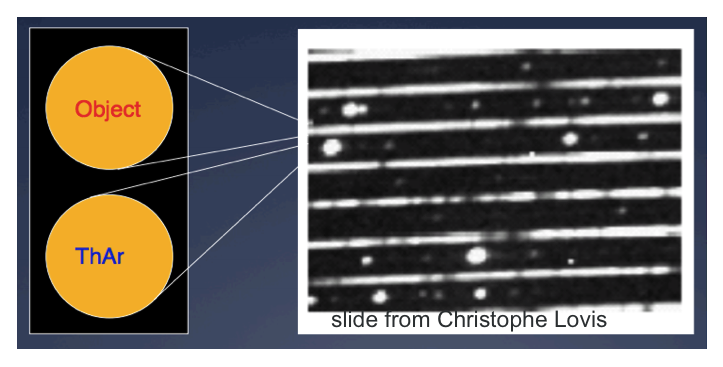
\includegraphics[scale=1]{introduction/thar.eps}}\
\subfloat[Iodine Cell on Lick/Hamilton]{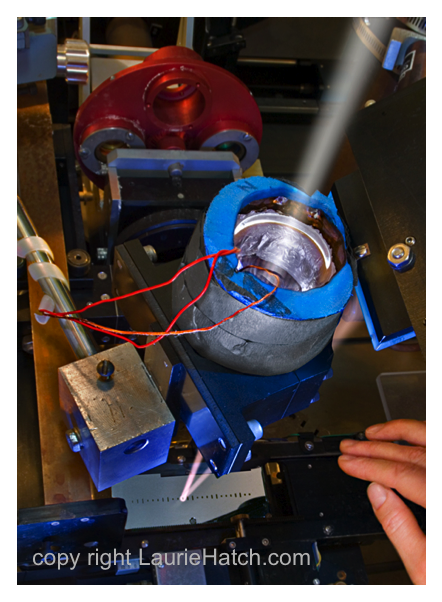
\includegraphics[scale=1]{introduction/iodine.eps}}
\caption{{\bf (a)} A portion of a HARPS-S spectral image as an
  example of ThAr calibrated spectrum. {\bf (b)} The Lick/Hamilton
  iodine cell in front of its slit plate.
\label{intro:fig:thar-iod}}
\end{figure}
%----------------------------------------------------------------


The pioneer work by zzz Campbell et al. calibrated their wavelengths
using an absorption gas cell filled with hydrogen fluoride (HF), which
provides well-known and clean and evenly (though sparsely) spaced
absorption lines in the red optical band. They were able to achieve a
stunning precision of 10-15~m/s back in the late 1980s. The discovery
of HD 114762$b$ by zzz Latham et al. at Harvard/CfA used the parallel
calibration approach, where they used solar spectrum at dusk and down
as calibrators. They later stabilized their spectrometer by employing
strategies such as mechanical temperature stabilization for the
spectrometer and fiber feeds and improved the precision to about 100
m/s.

The spectrometer Mayor and Queloz used to discover 51 Peg $b$ was
ELODIE \citep{elodie}, which achieved 15 m/s thanks to its excellent
mechanical stability. The Geneva team lead by Mayor and the European
community continued along the path with parallel calibrators (with
ThAr lamps in 4000-6900\AA) and stabilized spectrometers. More and
more exoplanet discoveries are made with two successors of ELODIE:
first CORALIE (1999), which achieved 2-7 m/s precision using
simultaneous ThAr calibration in the spectral image
(Figure~\ref{intro:fig:thar-iod}), and later on HARPS-S (2004;
\citealt{harps-s}), with its stunning stability of 1 m/s enabled by
its ultra-stabilized cryogenic enclosure. The European team later went
on to build HARPS-N (2012; essentially a copy of HARPS-S, with a RV
precision of 1 m/s) in collaboration with the Harvard/CfA group
including David Latham.

Meanwhile across the ocean, in the early 1990s, Geoffrey Marcy and
Paul Butler adopted the absorption gas cell approach and began their
survey on nearby solar type stars. Their choice of gas cell was the
iodine cell (Figure~\ref{intro:fig:thar-iod}), which had dense and sharp absorption lines across the
green part of the optical spectrum (5000-6200\AA), where it is also
rich of stellar lines for solar type stars. They first began with the
Hamilton spectrograph at Lick Observatory, which achieved 3-7 m/s zzz
Fischer paper. Later on, they achieved 1-3 m/s with HIRES on Keck I
(1996; then in 2004, a CCD upgrade brought the precision to 1-2
m/s). Chapter~\ref{chap:keck} is on improving the RV precision of
\keck. The surveys done by Cochran and Hatzes also used iodine
calibrators, first with the coud\'e spectrograph 2.1~m telescope at
McDonald Observatory (20 m/s using oxygen lines and later 10-20 m/s
with an iodine cell), then later on with HRS on the Hobby-Eberly
Telescope (HET) at the same observatory (3 m/s), whose
``under-performance'' in comparison to \keck\ is the focus of
Chapter~\ref{chap:het} of this thesis.

The efforts and instruments described above all operate in the optical
band. The RV precision in the near infrared (NIR) is about an order of
magnitude lower. zzz Barnes 2012, Blake 2010, and Figueira 2010a
demonstrated 5-20 m/s precision in the NIR using telluric lines as
wavelength calibrators. The ``state of the art'' for NIR precise RV in
2016 is the 5 m/s precision achieved by Bean 2010 zzz using CRIRES and
a methane gas cell as the calibrator. The two bottlenecks are hardware
stability and telluric contamination. Fortunately, with the cryogenic
NIR spectrometer CARMENES (whose commissioning has began in November
2015; it also has an arm in the optical band) and HPF (scheduled to
begin in 2016), the situation in the NIR will change quickly in the
very near future.

As of 2016, the precision of \keck\ and HARPS represents the state
of the art of the field. These two methods of wavelength calibration
have contributed almost equally to the ensemble of exoplanets
discovered using precise Doppler spectroscopy. There are, of course,
many other precise Doppler spectrometers that are running today, and
\cite{eprv2015} summarizes their performance in terms of RV
precision in details. Table 1.1 zzz summarizes these spectrometers and
their reported precision as in \cite{eprv2015}, which provides an
overview of the landscape of precise Doppler spectroscopy in 2016.

It took about a decade to breach the 10 m/s precision barrier
\citep{butler1996}, and optimistically, one would expect the 1 m/s
barrier to be breached a few years ago around 2010. Unfortunately,
this was not the case. Figure \ref{intro:fig:family} shows the
evolution of RV precision and how we have basically stalled around the
1-2 m/s level for the past two decades. Except for a couple of
extremely bright stars that were observed heavily with HARPS-S, there
has not been detections of planets regularly made with a precision
below 1 m/s. The reasons are complicated and many.

{\bf Stars} are known to be ``uncooperative'' in terms of staying RV
quiet. (1) The choice of stars is important, because magnetically
active stars such as giants and fast rotators are intrinsically tough
for precise RV surveys. There is also the concern of stellar
brightness, because the signal-to-noise ratio of the spectrum directly
affects the RV precision, which makes large telescopes such as Keck
and HET are more efficient for RV surveys. (2) Stellar activity
induced RV signals on the level of 1-2 m/s are very hard to model. The
physical mechanism behind such stellar jitter, such as macro
turbulence, is still relatively poorly understood, which makes stellar
activity arguably the most difficult piece in the puzzle of getting
down to 10 cm/s. We have some handle on spots or plague induced RV
signals (zzz cite Dumusque), and it is encouraging to see successful
cases such as CoRoT 7$b$ zzz Haywood, where the stellar RV signal is
neatly modeled with the help of photometric data and advanced
statistical tools.

{\bf Hardware stability} builds the foundation for high RV
precision. (3) Changes in temperature and pressure will induce mechanical
changes of the spectrometer and also change the index of refraction of
the air, and both will translate into wavelength solution drifts on
the CCD and thus RV noise. The successful story of HARPS has shown
that it is best to have an ultra stabilized spectrometer sealed in a
temperature and pressure controlled vacuum vessel. (4) Moreover, the light
going into the spectrometer needs to be stabilized, in the sense that
the fiber optics which feeds the spectrometer needs to be evenly
illuminated and stay stable (Halverson zzz). (5) Another extremely
important piece is the fidelity and stability of the wavelength
calibrator, and the next generation precise Doppler spectrometers are
all making the switch from using ThAr lamps to laser frequency combs
zzz citation. Chapter~\ref{het:sec:fts} shows the importance of the
stability and a full knowledge of the iodine cell to RV precision.

{\bf Elimination of telluric contamination and robust data analysis
tools} are crucial ``software'' aspects that ensure the delivery of
high RV precision out of the raw spectral data. (6) As mentioned
above, telluric contamination is a bottleneck for NIR precise RV, and
it has not been considered a problem for the optical RV community
until recently because it contributes to the RV error budget by about
10-50 cm/s, well below the current precision (see more in
Chapter~\ref{keck:sec:telluric}). (7) Robust data analysis tools are
also crucial because it is the last avenue for battling instrumental
and stellar RV systematic errors. For the ThAr calibrated spectra,
precise RVs are measured via cross correlation between a ``mask'' with
varying weights at the positions of stellar lines and the observed
stellar spectrum that are flattened and wavelength-calibrated zzz
citation. For iodine calibrated spectra, precise RVs are extracted
through the forward modeling method, which is described in detail in
Chapter~\ref{chap:doppler} and is also the theme for
Chapter~\ref{keck:sec:dsst} and \ref{keck:sec:algorithm}. Interpreting
the RVs and translating them into planetary orbits is also challenging
and crucial (Chapter~\ref{chap:boottran}), especially with the
existence of stellar activity induced signals zzz cite alpha cen.

Here I have only briefly discussed each item, with the goal to present
a broad picture of how precise Doppler spectroscopy works and provide
a general background for this thesis. For a more detailed description
and summary of the status and the community's plans on breaching the
10 cm/s barrier, see \cite{exopag2015} and \cite{eprv2015}. A list of
future precise Doppler spectrometers is presented in Table~1.2 zzz,
and most of them have a target RV precision of below 50 m/s or even 10
cm/s.


%----------------------------------------------------------------
% RV K vs. year
% plot generated on exoplanets.org and hand edited for 2015 postdoc proposals
% copied over from ~/Jobs/plots/
\begin{figure}
\centering
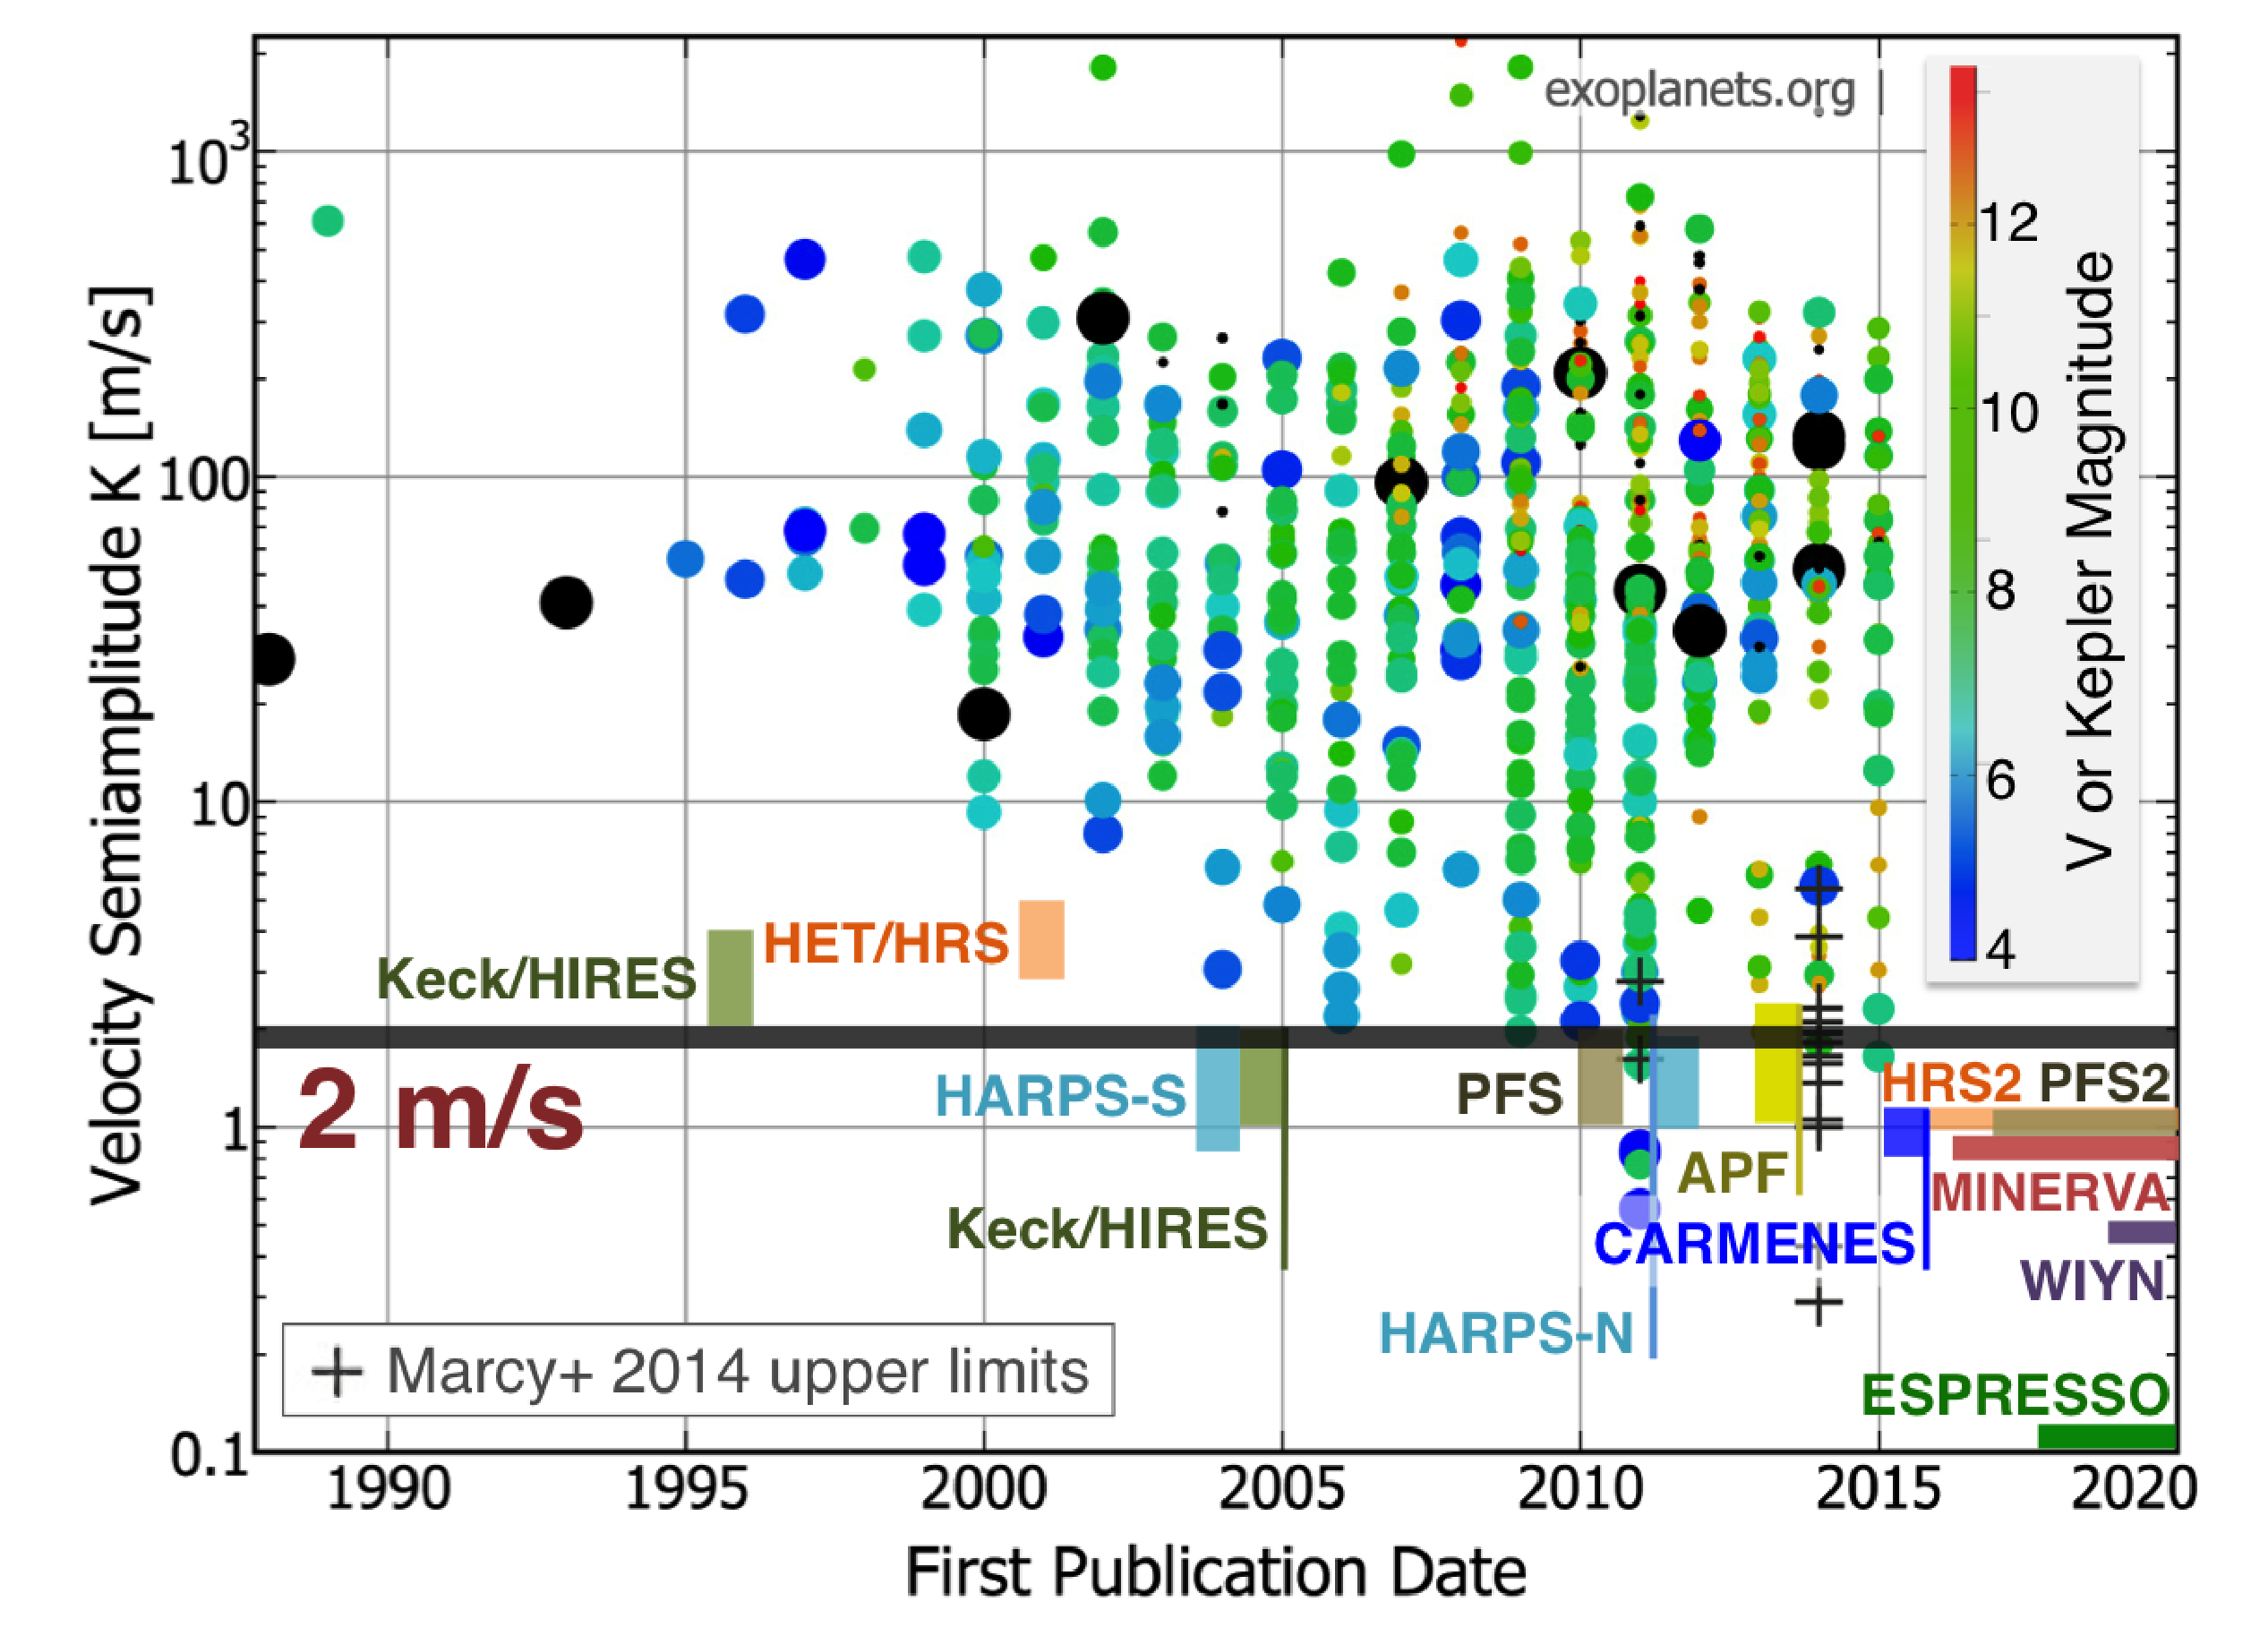
\includegraphics[scale=0.32]{introduction/family-big-carmenes.eps}
\caption{The RV semiamplitude $K$ of all RV-detected exoplanets
  vs. date of discovery. The planets are color- and size-coded according
  to their host star brightness. The RV precision has essentially
  stalled at $\sim$2 m/s level since 2005, except for a very few bright
  stars observed with high cadence. Current major RV instruments are
  plotted at their start dates, with the position and height of the
  rectangles indicating their RV precision. Selected future RV
  instruments are labeled in thick lines showing their first-light dates
  and target precision. The black crosses are the \kepler\ small planets
  with mass upper limits in \cite{marcy2014} measure by \keck.
\label{intro:fig:family}}
\end{figure}
%----------------------------------------------------------------



%%%%%%%%%%%%%%%%%%%%%%%%%%%%%%%%%%%%%%%%%%%%%%%%%%%%%%%%%%%%%%%%%%%%%%%%%%%%%%
\section{Precise Doppler Spectroscopy with Iodine Cells as
  Calibrators, and an Outline for This Thesis} 

Precise Doppler spectroscopy with iodine cells as calibrators has had
a glorious past full of exciting discoveries, such as the first stars
with multiple planets \citep{butler1999}, the first Earth-size
Earth-mass planet \cite{howard2013, pepe2013}, and also the
characterization of first sample of sub-Neptune and super-Earth
planets (\citealt{marcy2014}) which enabled the first studies on the
demographics of small exoplanets zzz. However, all future precise
Doppler spectrometers are going to be ultra-stabilized and calibrated
by laser combs with $<$1 m/s precision. How would
iodine-calibrated Doppler spectrometers such as \het\ and \keck\ fit
into the current and future pictures of precise RV?

First, the iodine-calibrated method is a relatively cheap way of
measuring RVs precisely at the 1-2 m/s level, because it does not
require pairing with a ultra-stabilized spectrometer like HARPS. Even
with the existence of Doppler spectrometers with $\sim$10 cm/s
precision, instruments with 1 m/s precision will still have plenty of
science to do such as RV follow up of transiting planets and
asteroseismic studies (e.g., the SONG telescopes, zzz). 

Second, iodine-calibrated instruments will stay competitive in the
next 3-5 years, especially during TESS era, because most 10-meter
class telescopes will only have iodine-calibrated precise Doppler
spectrometer (the only exceptions are HPF on HET in the NIR and
ESPRESSO on VLT). There are several next-generation spectrometers
being built or planned for large telescopes such as iLocator,
MAROON-X, and SHREK (Table 1.2 zzz), but it is unlikely that they
would be scientifically competitive during most of the TESS mission
era. Large apertures are highly desirable for \kepler\ and TESS follow
up. For example, HARPS-N can only target stars brighter than the
10$^{th}$ \kepler\ magnitude, while \keck\ can follow up an order of
magnitude more (median brightness for \kepler\ stars is about 13-14
mag). As a result, majority of the \kepler\ RV follow up is done by
\keck. Even for TESS, which primarily target ``bright'' stars, the
median $V$ magnitude for Sun-like stars is actually below 11. It is of
no doubt that \het\ and \keck\ will play an important role in TESS
follow up.

Improving the precision of \het\ and \keck\ will enable more efficient
follow up on TESS targets and also benefit the independent long-term
RV surveys being carried out at HET and Keck. This is the goal of this
thesis. Improving the precision of the fiber-fed \het\ also helps us
to gain a better understanding on modeling fiber-fed instruments and
to prepare for future ones such as MINERVA \citep{minerva}. The work
in this thesis will also improve the RV precision on archival \het\
and \keck\ data, which span over a decade -- the longest baseline in
the history of precise Doppler spectroscopy. 

The scope of this thesis is mostly on RV data analysis, including
improving the data analysis tools and diagnosing hardware problems
through data. Chapter~\ref{chap:doppler} contains the documentation on
the software package I used for getting RVs out of \het\ and \keck\
data, and it also serves as an introduction on extracting RVs from
iodine-calibrated stellar spectra. Chapter~\ref{chap:het} and
\ref{chap:keck} document my efforts in improving the RV precision of
\het\ and \keck, respectively. The introduction sections in these two
chapters contain more information on these two instruments and a
general background on my work. Chapter~\ref{chap:boottran} and
\ref{chap:planets} are from peer-reviewed, published
papers. Chapter~\ref{chap:boottran} documents my work in
characterizing exoplanet orbits using RV data, and
Chapter~\ref{chap:planets} reports the discovery of HD 37605$c$, which
is the first exoplanet discovered by the Wright
group. Chapter~\ref{chap:conclusion} contains a brief summary of the
findings in this thesis and a description of future directions beyond
the ones mentioned in its preceding chapters, where the readers will
see that the toolset built for this thesis and the lessons learned on
how to model the stellar spectra precisely are valuable not only for
iodine-calibrated data, but also for general future works on detecting
new worlds using precise Doppler spectroscopy.
